\subsection{Target Areas in the Gulf of California and Dataset Statistical Analysis}
\begin{figure}[t]
    \center
    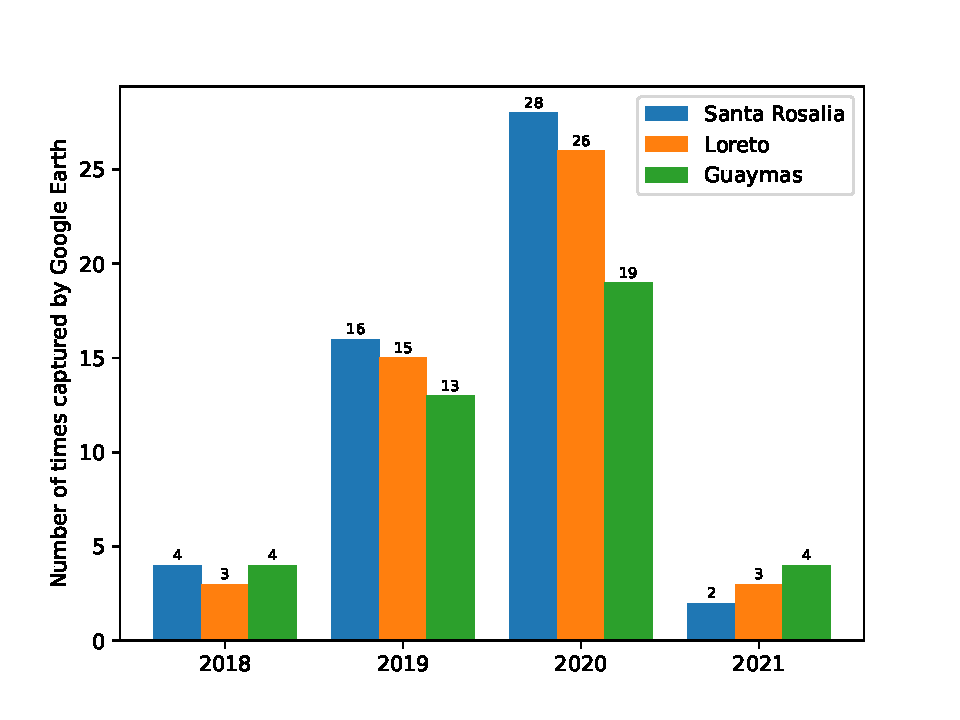
\includegraphics[width=\columnwidth]{img/NumberOfTimesCapturedByGEP.pdf}
    \caption{Number of times the three cities (Santa Rosalia, Loreto, Guaymas) captured by Google Earth Pro from 2018 to 2021.}
    \label{NumberOfTimesCapturedByGEP}
\end{figure}

The Gulf of California in Mexico was chosen as an area of study. Ideally, to analyse a sufficient amount of satellite image data, the ports of each of the major harbour cities in the Gulf of California would need to be included in the scope of our study. Thus, the first step in this work was to determine if there was enough satellite data for the area. In this study, the Gulf of California was split into a few zones based on the Mexican state limits: (1) Baja California, (2) Sinaloa, (3) Sonora, and (4) Baja California Sur. The satellite dataset used in this analysis included 694 high-resolution (4800 pixels x 2908 pixels) images of ships worldwide collected from Google Earth~\cite{lutherborrowship}. From the imagery dataset, a statistical analysis was performed on how many times, temporally speaking, the satellite database captured the region of interest. As a result of this analysis, it was found that:
\begin{itemize}
    \item most cities in the Gulf of California do not have enough satellite data in 2018 and 2021, while many cities have relatively rich satellite data between 2019 and 2020;
    \item there has been a steady increase in the collection of satellite data in the Gulf of California from 2018 to 2020;
    \item the open-access and high-quality satellite data from Google Earth Pro is not immediately available to the public;
    \item differences in data accessibility are still evident among different cities. For example, Guaymas in the state of Sonora has rich satellite images in 2019 and 2020. However, other cities, such as La Ventana in the state of Baja California Sur, did not appear on Google Earth Pro between 2019 and 2020.
\end{itemize}

\begin{figure}[!t]
    \center
    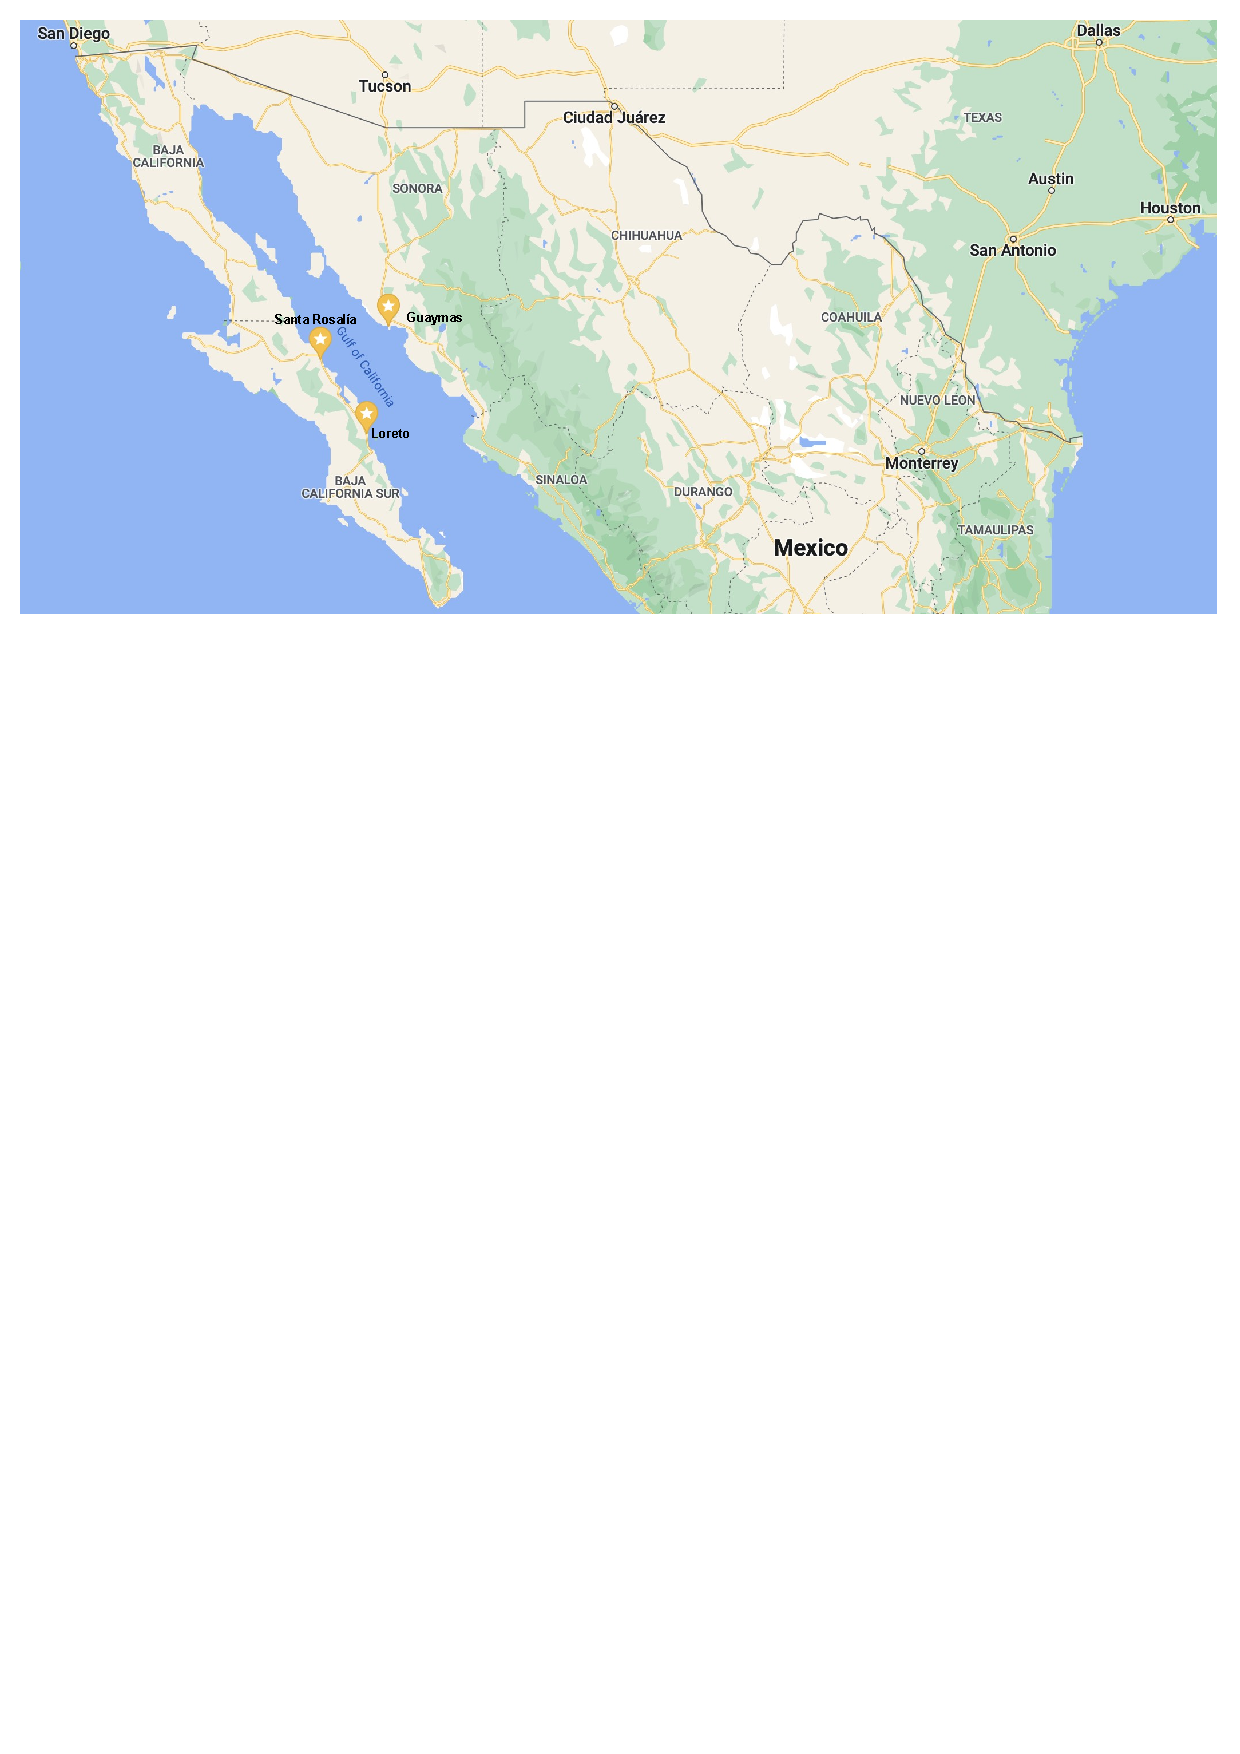
\includegraphics[width=\columnwidth]{img/locations_maps.pdf}
    \caption{The geographic locations of the three target cities - Santa Rosalia, Loreto, and Guaymas - in Google Maps.}
    \label{locations_maps}
\end{figure}


For this reason, continuing with the previous strategy of analysing the satellite data for each city in the Gulf of California would lead to a relatively large information bias and thus would not achieve an effective object detection model. Therefore, the following three cities with the richest data-accessibility in Google Earth Pro were chosen as the target areas for this study: Santa Rosalia, Loreto, and Guaymas (see Figure~\ref{locations_maps} for their geographical locations). The number of times captured by Google Earth Pro~\cite{lisle2006google} is shown in Figure~\ref{NumberOfTimesCapturedByGEP} with a database of 583 images with timestamps between 2019 and 2020 for the three Mexican coastal cities.


\subsection{Preprocessing}
Each satellite image was manually pre-labelled with a highly-precise label box ~\cite{lutherborrowship}. The original dataset contained images larger than 9 MB, which is an efficiency burden for neural network training, especially when few objects are detected. For this reason, all images were resized from 4800 pixels x 2908 pixels to 416 pixels x 416 pixels, with the file sizes reduced to between 10KB and 40KB~\cite{nelson_2020}. 


\subsection{Single Object Detection Architecture}
\label{III-D-Detection-Architecture}

Figure~\ref{model_architecture} shows a schematic of the models being used for detecting boats, where satellite images in the Gulf of California are the input of a pre-trained convolutional neural network (CNN). The detection accuracy was determined by computing the mean probability score from the Gulf's satellite images. In Sec~\ref{sec2.2}, recent literature and the development of Convolutional Neural Networks (CNNs), including the YOLO model, were discussed. YOLOv5 has four different categories of models, YOLOv5s, YOLOv5m, YOLOv5l, and YOLOv5x~\cite{glenn_jocher_2022_6222936}. They have 7.3 million, 21.4 million, 47.0 million and 87.7 million parameters, respectively. The performance charts can be seen as Figure~\ref{fig:YOLOv5_Performance} where the YOLOv5l model can achieve higher average precision with the same faster computing speed. Thus, in this study, the YOLOv5l model was chosen as the model for the training dataset.

\begin{figure*}[!t]
    \centering
    \includegraphics[width=7in]{img/model_architecture.pdf}
    \caption{\textbf{Model architecture.} Detection model architecture for obtaining a conclusion from an input satellite image of boats.  Images are preprocessed and passed through a CNN. The model's output is a score, $y \in (0,1)$, representing the probability of being detected as a boat.}
    \label{model_architecture}
\end{figure*}

\begin{figure}[!t]
    \center
    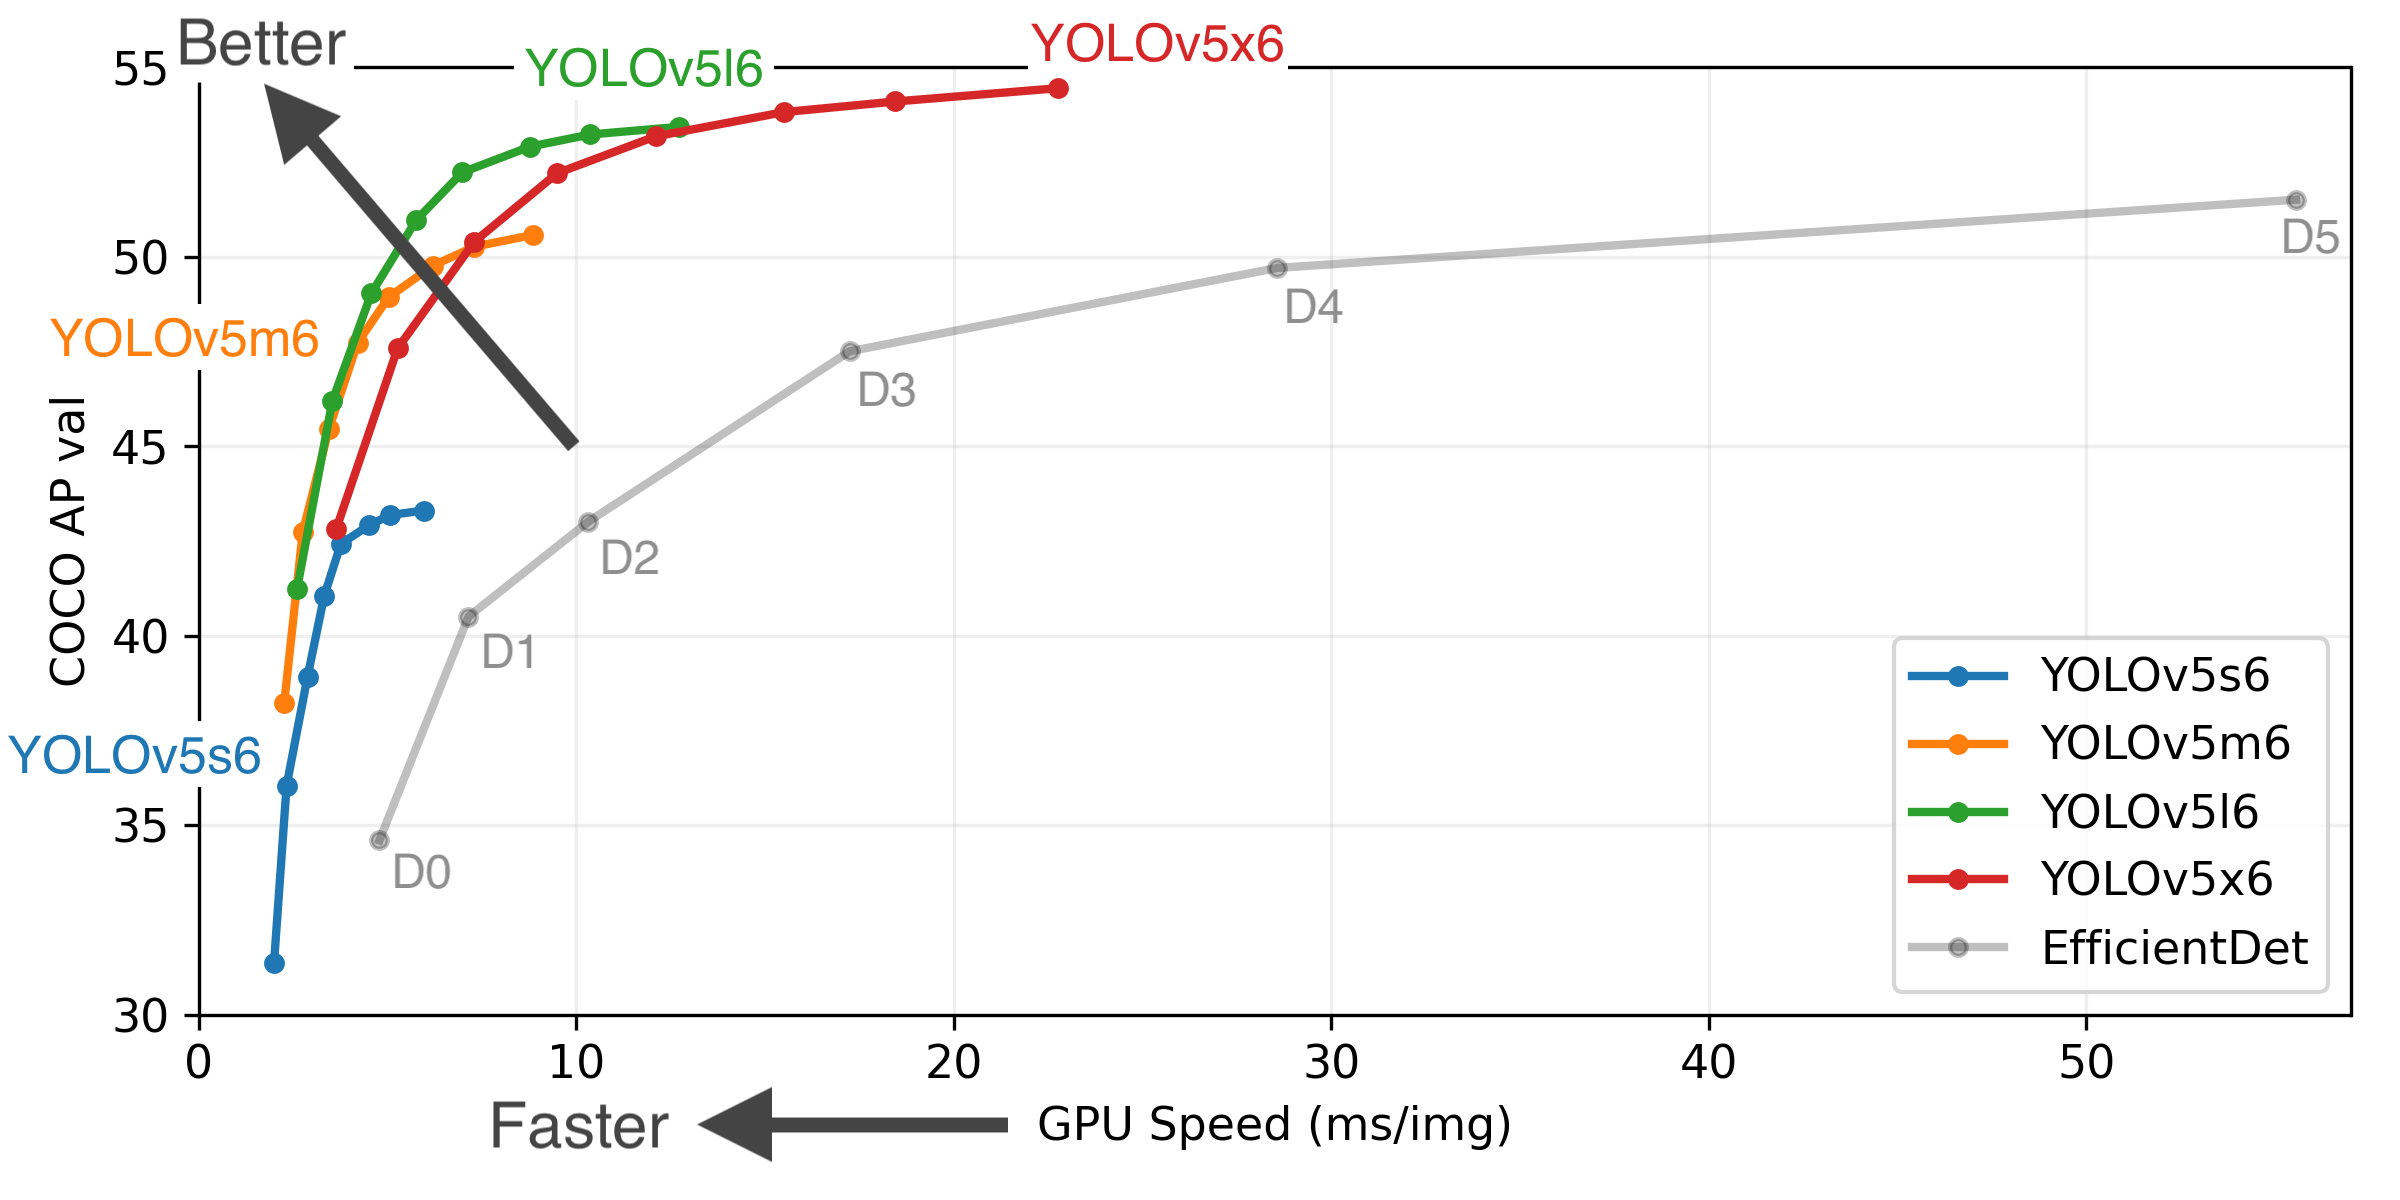
\includegraphics[width=\columnwidth]{img/YOLOv5_Performance.png}
    \caption{{Average Precision (AP) vs GPU Speed in the 6th generation of YOLOv5 model under COCO data set~\cite{glenn_jocher_2020_4154370}.}}
    \label{fig:YOLOv5_Performance}
\end{figure}


Satellite images often contain noise such as shadows cast by water on the sea surface or clouds in the atmosphere, which make the training data inaccurate and often cause problems ensuring the model's correctness. He et al.~\cite{He2009SingleIH} proposed a simple but effective image prior-dark channel before removing haze from a single input image. The prior-dark channel can be used as a statistic of outdoor haze-free images. Based on critical observation, most local patches in outdoor haze-free images contain some pixels whose intensity is very low in at least one colour channel. Using this prior-dark channel before the haze imaging model, the thickness of the haze can be estimated, and a high quality haze-free image can be recovered. Moreover, a high quality depth map can also be obtained as a byproduct of haze removal.

Similar to the principle of using convolution kernels, specific image kernels can sharpen the image. While the sharpening kernel does not produce a higher resolution image, it emphasises the differences in adjacent pixel values, making the image appear more vivid. Overall, sharpening an image can significantly improve its recognition accuracy with a 5x5 image kernel.

\subsection{Object Measurement and Classification}
Measuring the length of a ship is one of the most challenging topics in this study. As Google Earth Pro does not provide an application programming interface (API) for accurate scales, manually measuring the size of a particular scale became the core process to calculate the size of any given ship. All of the captured satellite images in this research were set with a fixed eye altitude. By measuring only one real length of the object through the Google Earth Pro measurement tool and knowing the pixel length of this object, the length of one pixel in the satellite image of the fixed eye altitude can be calculated.

As the dataset for the training model was created with each edge tangent to the edge of the detected object, it can roughly treat the boat's length as the length of the diagonal within the detection box. Secondly, since the scale is central to the detection of the small boat fleet, the imagery scale should follow the following rules:
\begin{itemize}
    \item cannot be too large. The image should contain the full area in which boats may be found.
    \item cannot be too small. If this is not followed it is highly probable that the group of boats are detected as a single but larger boat.
    \item be sufficiently clear. This characteristic allows the algorithm to quantify the boat's length and accurately classify the measurements.
\end{itemize}


The eye altitude was set to 200 metres based on the above rules. This study used a satellite image of Zurich Lake, Switzerland, on 16th August 2018 as the standard image for defining the scale (Figure~\ref{fig:zurich}). Compared with other regions, the satellite image of Zurich Lake complies with the rules, and it is a suitable candidate as the standard for measuring the length of small boats. This standard was then used for the rest of the imagery database.

\begin{figure}[!t]
    \centering
    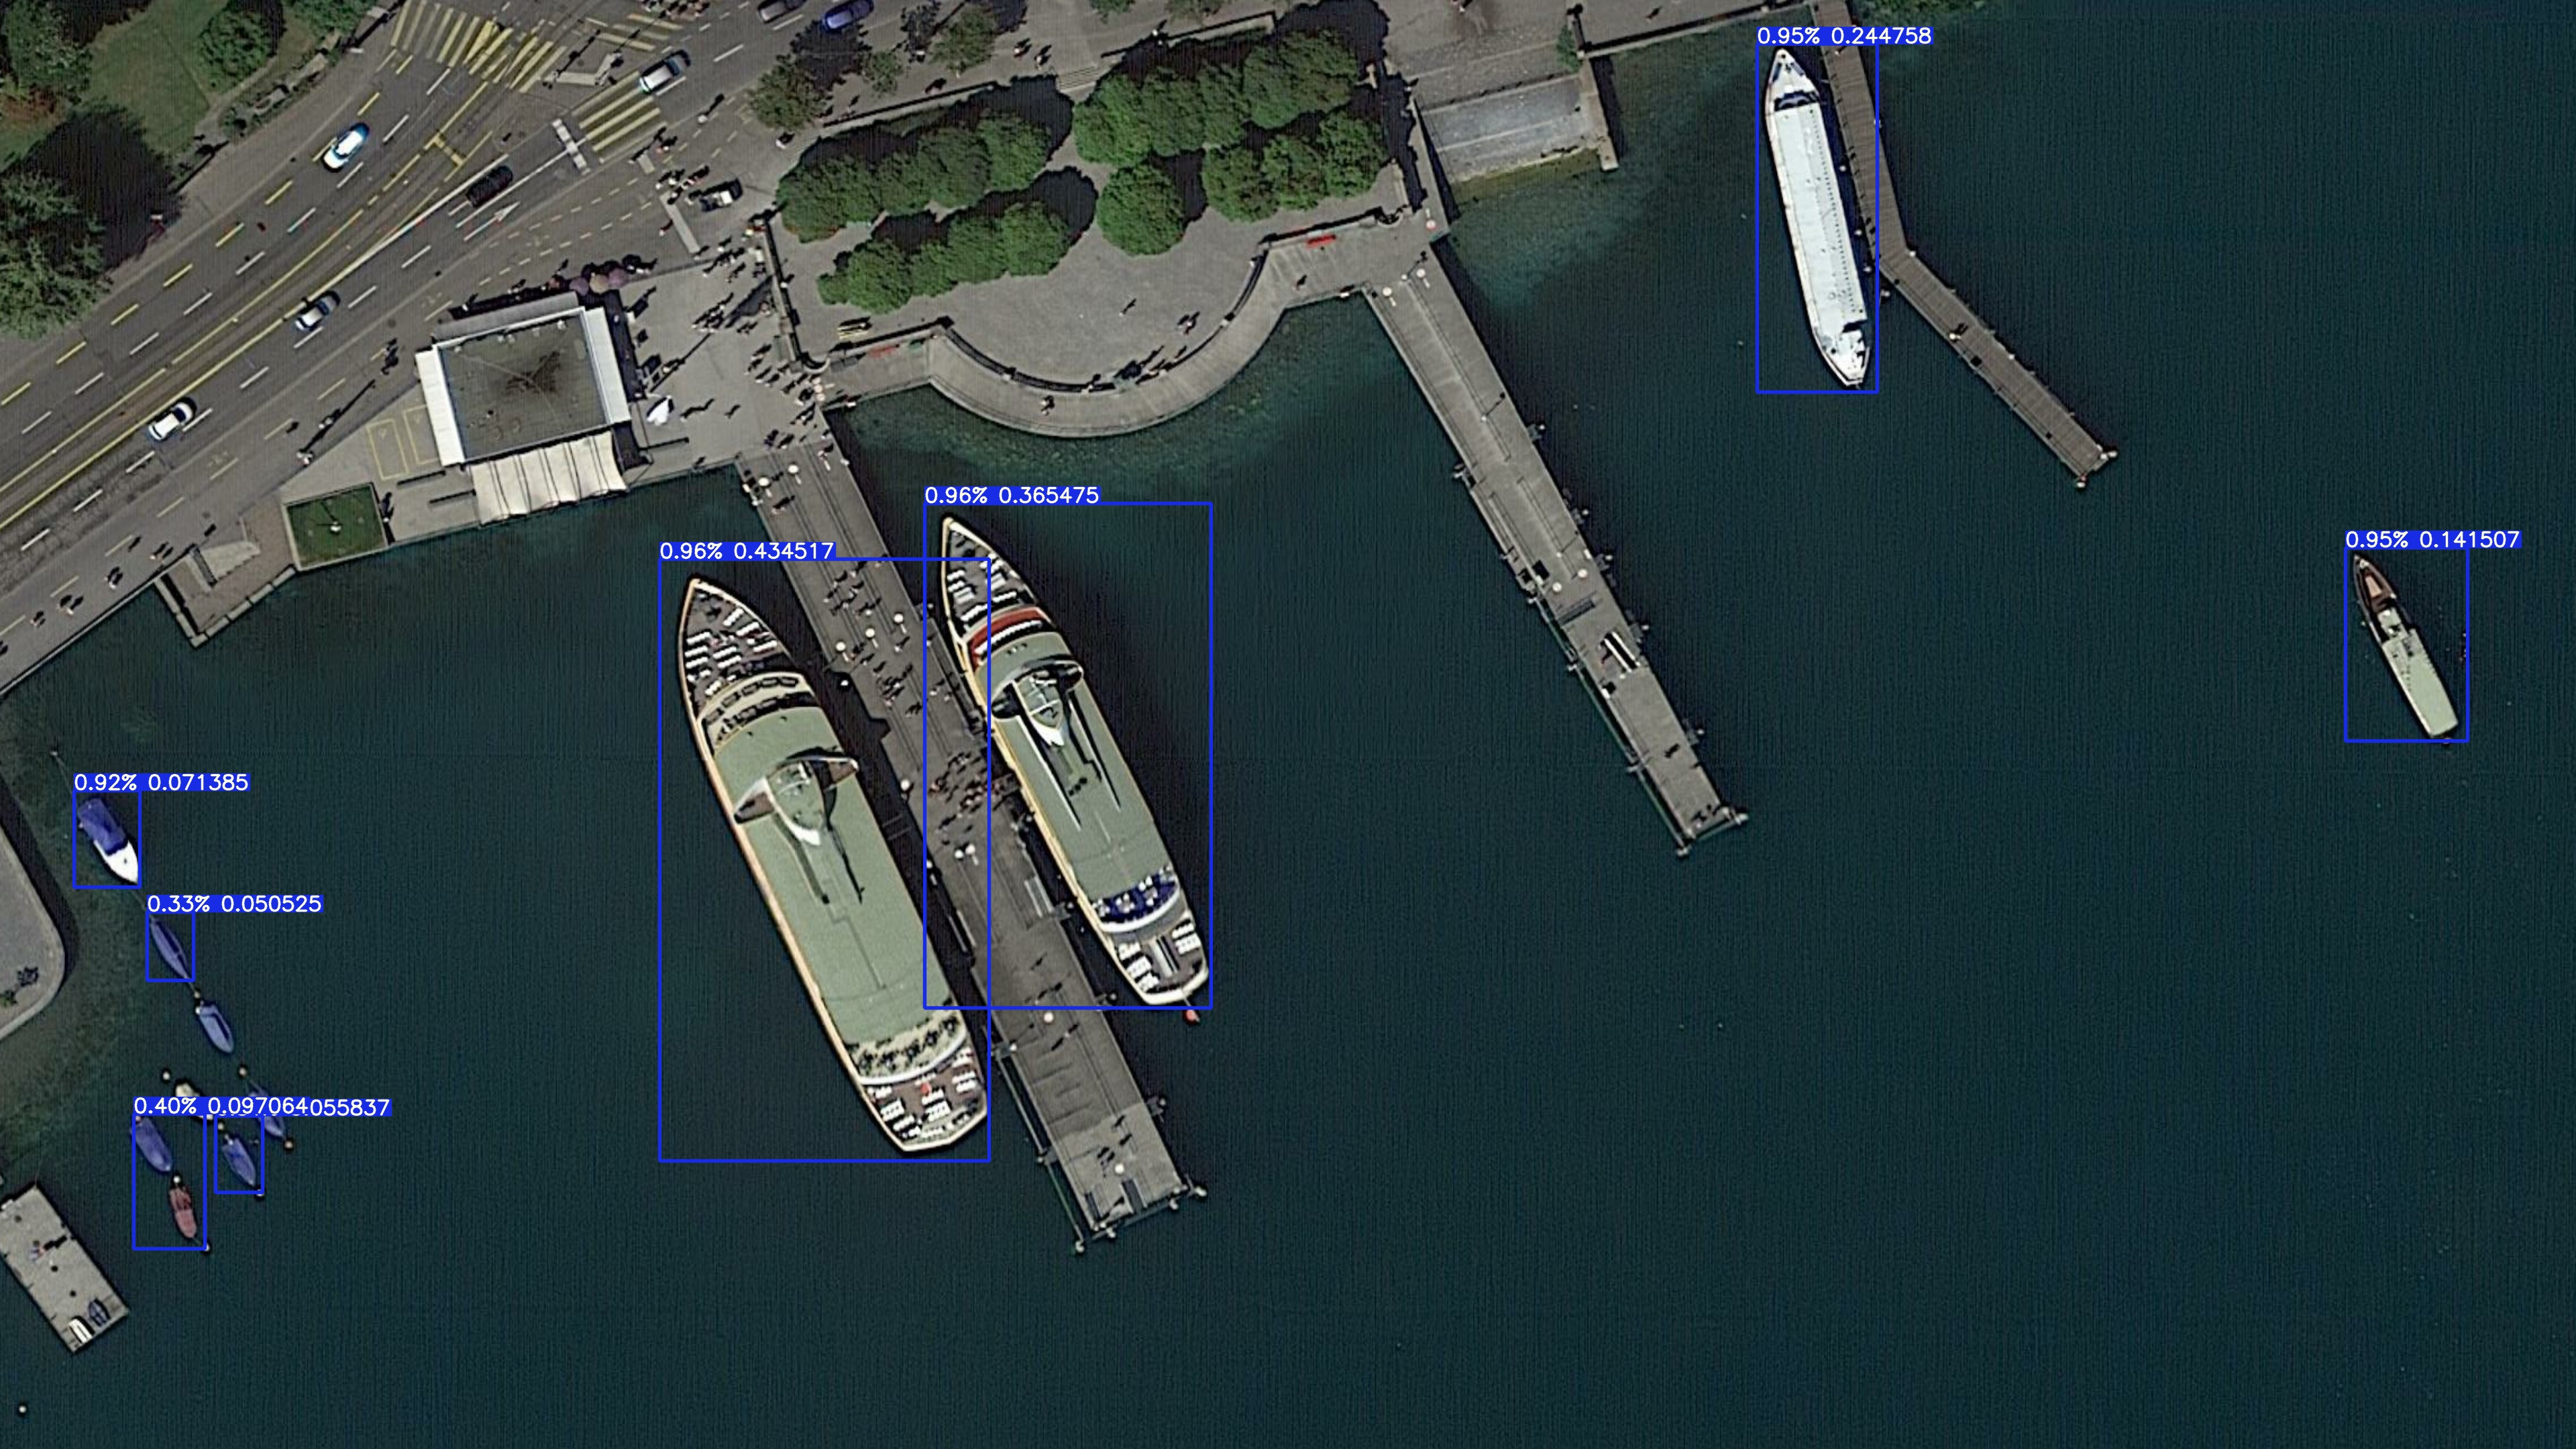
\includegraphics[width=\columnwidth]{img/zurich.jpeg}
    \caption{An image from Google Earth Pro for Zurich Lake on 16 Aug 2018 when eye alt is 200 metres.}
    \label{fig:zurich}
\end{figure}

After measurement, the vessel in Figure~\ref{fig:zurich} had a YOLO length of 0.43 that, after the scale conversion, represented 55.17 metres. With an eye altitude of 200 metres, the ratio of the absolute length to the YOLO length was approximately 127. Finally, after several verification tests, this ratio returned a small margin of error (around 1\% to 3\%) and hence was deemed a suitable scaling ratio for the remaining images. Moreover, having the same ratio and eye altitude was not enough. The resolution of each image must be the same, so measurements are standardised. For this purpose, all datasets that detect small boats will maintain a resolution of 3840x2160 pixels.

In a certain sense, large vessels (e.g. cargo ships) and small vessels (e.g. small boats for domestic use) are distinguished when creating the dataset for the area of interest. However, due to the scaling, some large vessels such as general cargo ships do not appear fully in an image. Hence they are not considered in the statistical results of this work. On the other hand, some of the larger vessels, slightly shorter in length than the 200m eagle eye scale, are identified correctly by the algorithm and counted as part of the number of large vessels in the area. A Python script was then designed to count the number of small and large boats between regions.

After distinguishing between large and small boats, it is necessary to distinguish between small recreational boats for domestic use and fishing boats without a roof. The model used the detected deck colour of the small boat to distinguish between them. If the deck was predominantly white, it was assigned a recreational boat, while any other mix of colour would be designated a fishing boat. It is recognised that this is a broad and simplistic classification method, but it is an effective one to test the categorisation power of the model. Each of the detected boats (i.e. the objects within the four coordinate anchor box) were analysed whether the colour was white or mainly white to assign it to each category. As a final step, the model performed the category counting for each image, where a Python script was designed to count the small white boats.
